
\item A bola de \SI{0.5}{\kilogram} de dimensão desprezível é lançada para cima na pista circular lisa usando o pistão com mola. O pistão mantém a mola comprimida \SI{0.08}{\meter} quando $s=0$. Determine até que $s$ ele deve ser puxado para trás e solto de maneira que a bola vá começar a deixar a pista quando $\theta=\SI{135}{^{\circ}}$.

\import{answers/}{answer-1}

\vspace{-1.5cm}
\begin{flushright}
    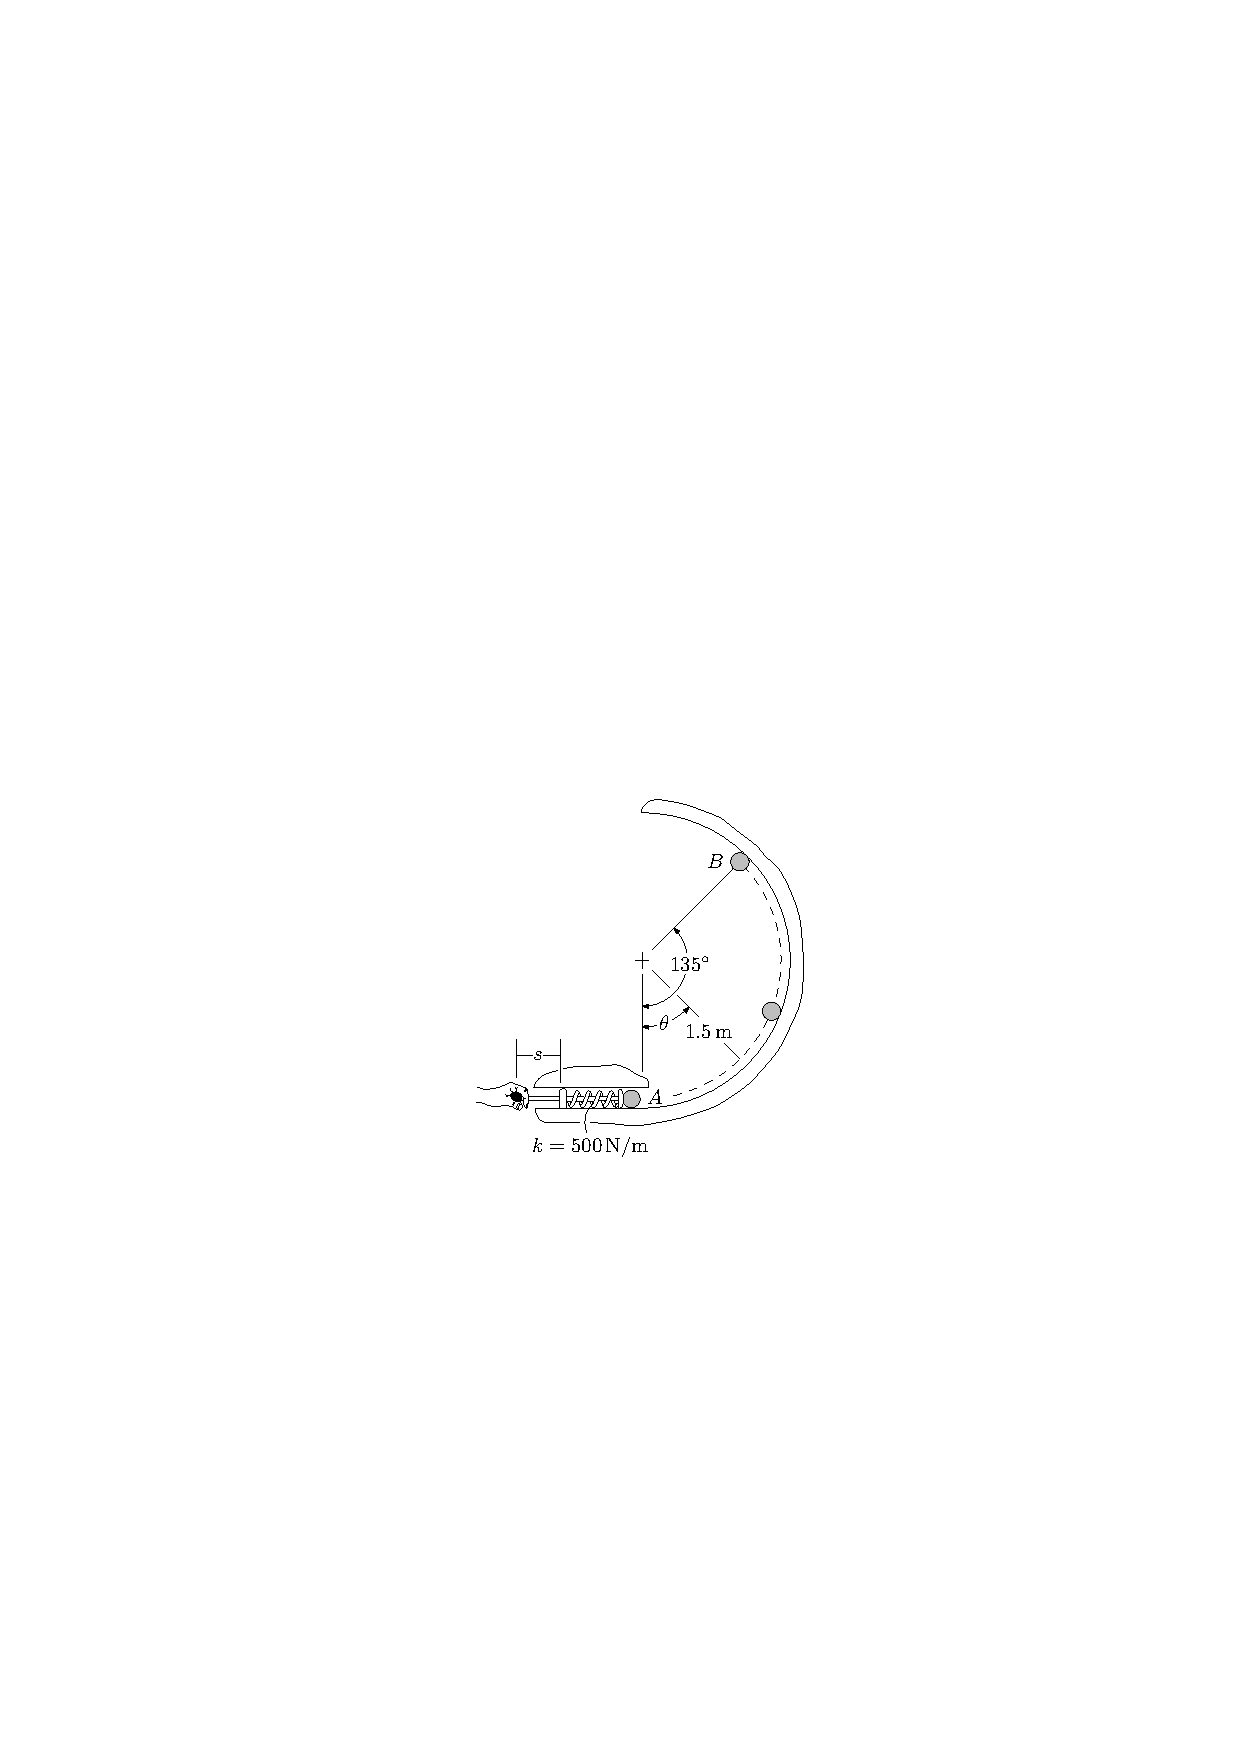
\includegraphics[scale=1.2]{images/draw_1.pdf}
\end{flushright}